\documentclass[a4paper]{article}

\usepackage{parskip}
\usepackage{setspace}
\usepackage{fullpage}
\usepackage{graphicx}
\usepackage{float}
\usepackage[justification=centering]{caption}


\begin{document}

\title{Product Management, Feedback and Evaluation}
\author{Andrew Higginson \and Bryan Liu \and Jia Guang Choo \and Emma Hulme \and 
Timothy van Bremen \and Thomas Taylor-Hall}
\date{\today}
\maketitle

\setcounter{table}{0}
\linespread{1.15}

\section{Project Introduction}

As part of the renovation of the William Penney Building on the Sherfield walkway, interactive screens are to be installed. Mounted inside the building, four projectors will simultaneously display content onto floor to ceiling glass panels that are visible to passers-by. Also, an 84-inch 4K resolution touch screen is to be mounted by the entrance doors. 

Our project consists of developing an ``App Store" for uploading interactive content and visualisations to be displayed on the four projected screens. Administrators will also be able to use this system to moderate and schedule content. Finally, we will be developing a playout system to show the content on multiple screens in multiple resolutions.

\section{Stakeholder Relationships}

\subsection{Stakeholders}

The main stakeholder in our project is our supervisor, David. The core of our project is the scheduling component, which he will operate as an administrator, so his opinion of the overall design of the project is critical.

Our second class of stakeholders are those who browse the visualisation catalogue and submit visualisations and advertisements. Their stake is relatively large as without their full engagement and satisfaction, the variety of content being shown will remain small. 

Our last group of stakeholders are those who see the visualisations being played out. While this set of users are still important, their stake is relatively small, in that all they want to see is the content being played out successfully.

\subsection{Customer relationship}

Where customer relationships are concerned, we see our most important stakeholder, our supervisor, David, as somewhere between an internal and external customer, whom we hold weekly meetings and exchange emails frequently with but not contact in person daily. During weekly meetings, we explain the features that are in progress/to be done over the next week, so that David is always kept in the loop (Figure \ref{fig:meetingboard}).

We tended to keep discussions fairly high-level, and only discussed implementation details/technologies when asked to do so, or when we felt that it was important to the discussion. We did this to mimic the scenario of David being our client, but also to ensure that discussions were not biased towards any kind of implementation, allowing us to fit our implementation around the best ideas, and not the other way around.

\begin{figure}[H]
  \begin{minipage}{0.49\textwidth}
    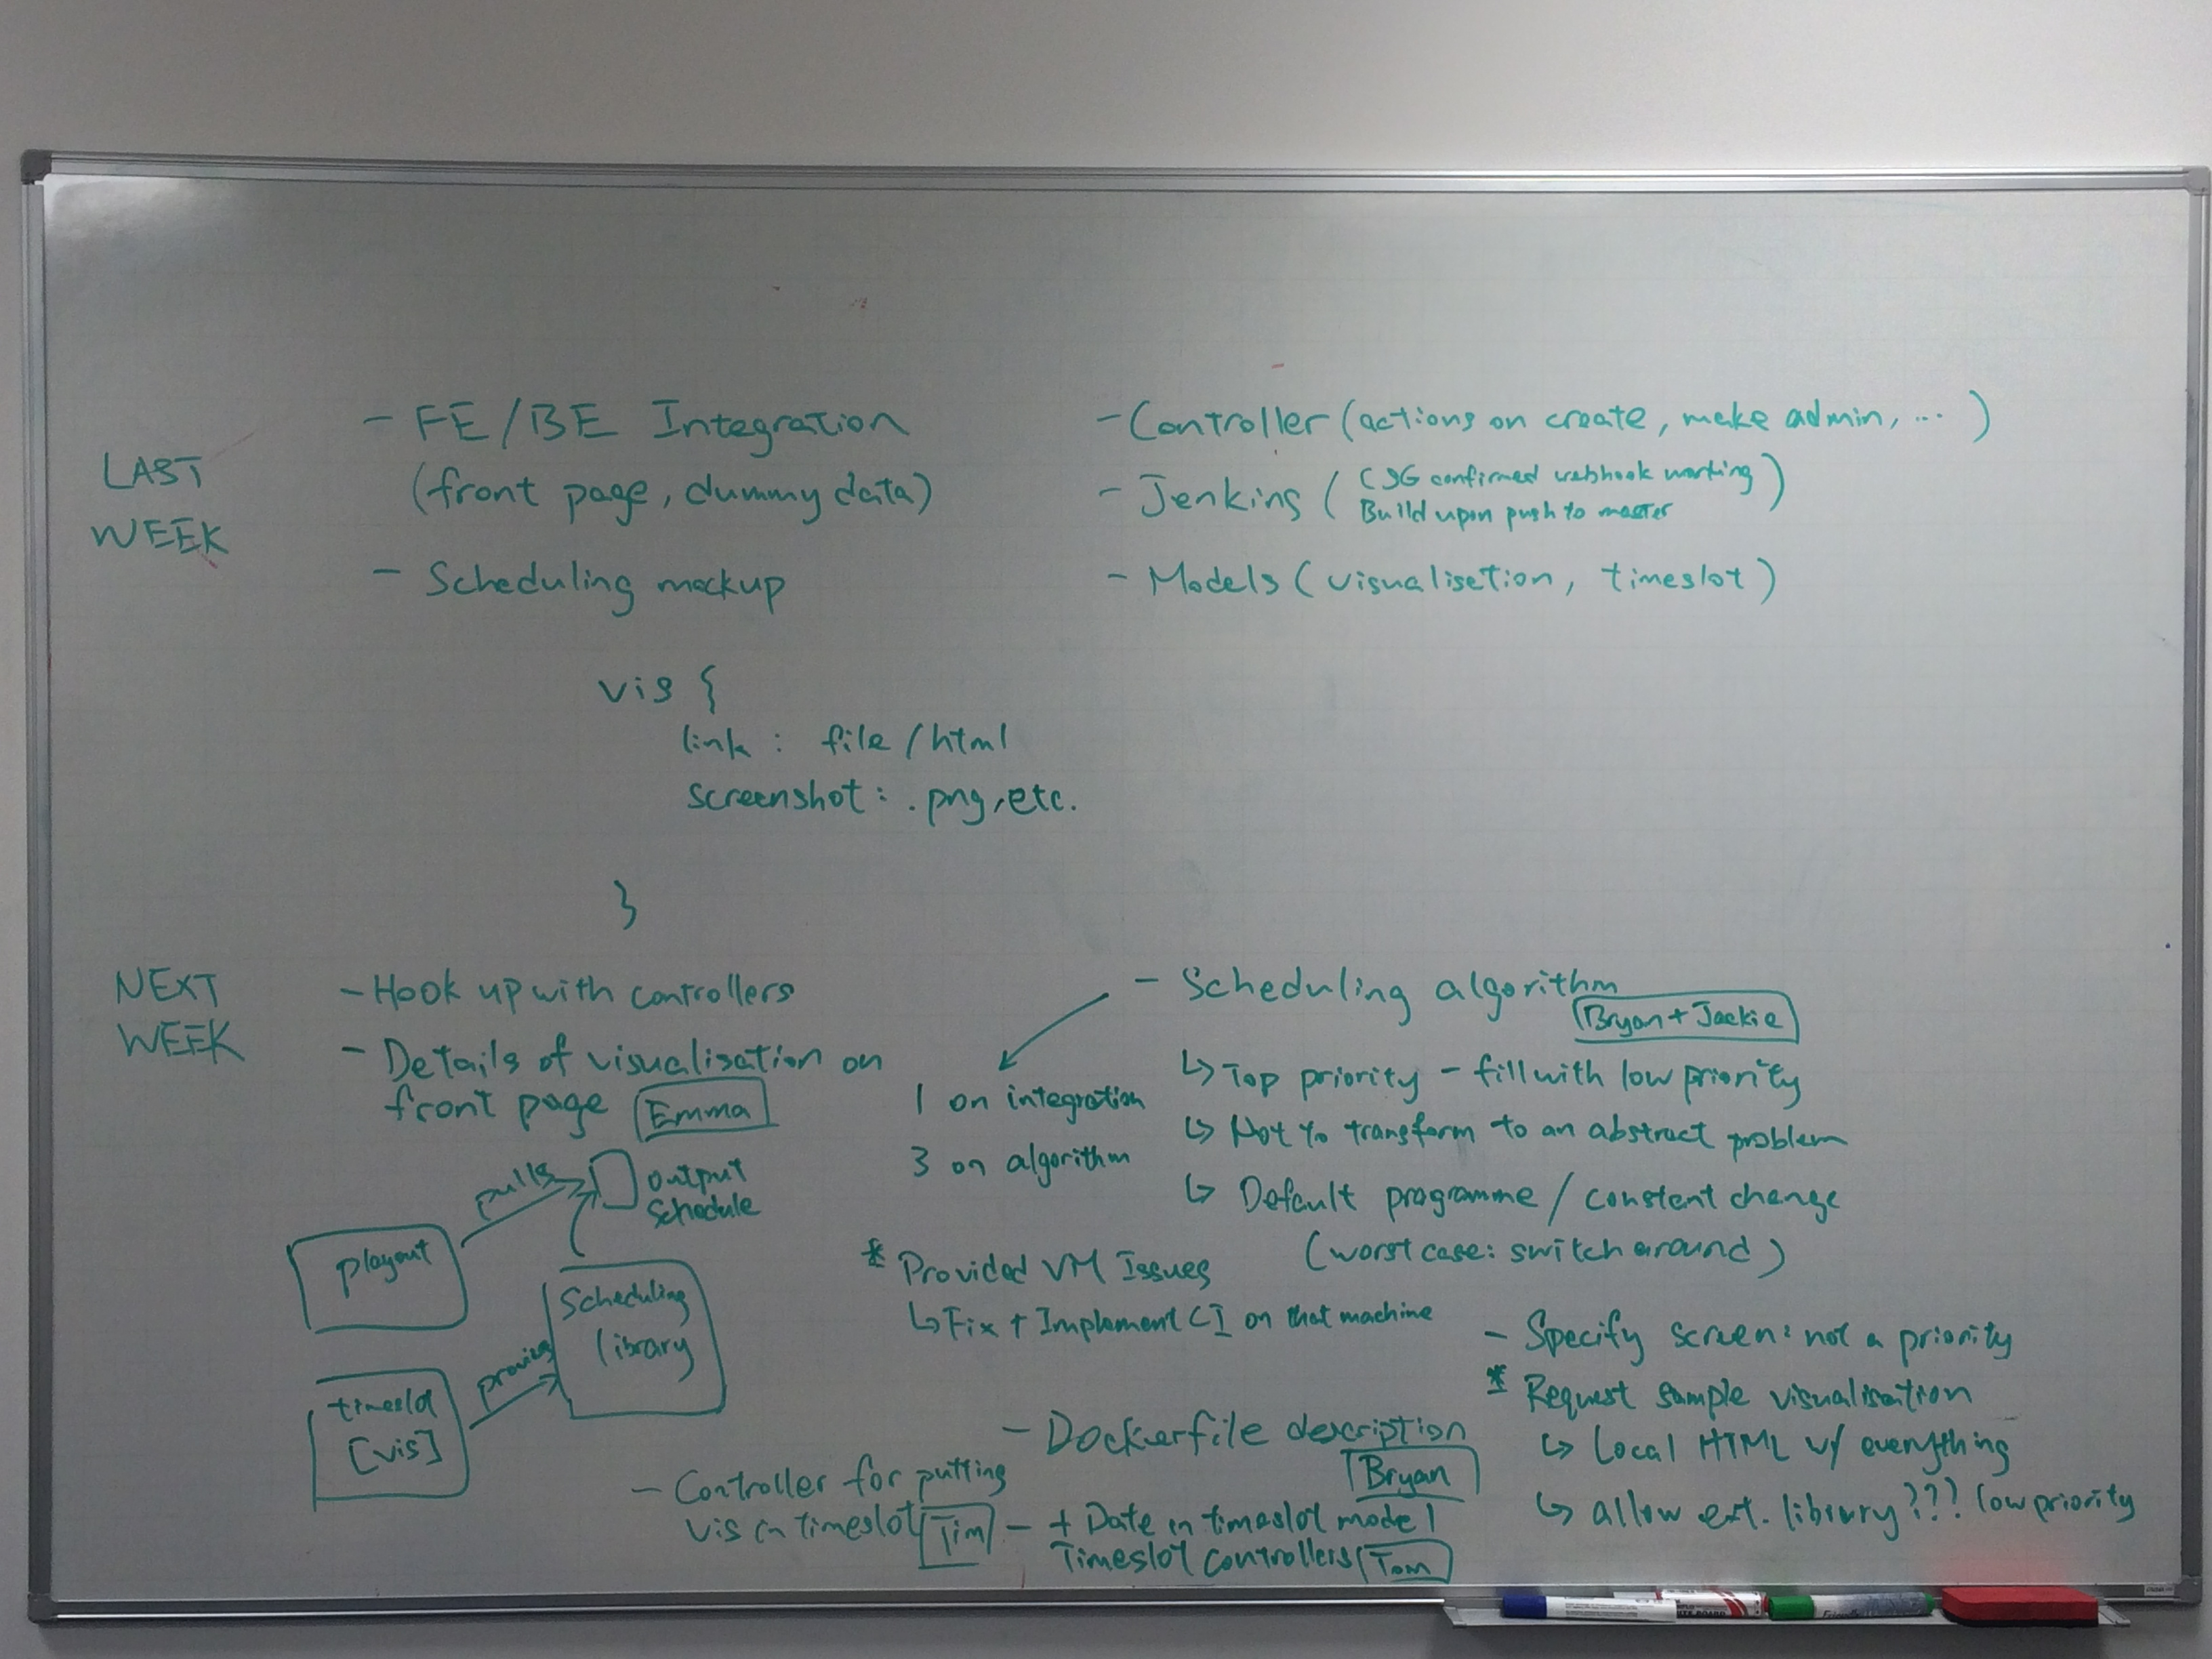
\includegraphics[width = \textwidth, trim = 0 0.4cm 0 1.6cm, clip]{./evaluation/meeting-board2.jpg}
  \end{minipage}
  \begin{minipage}{0.49\textwidth}
    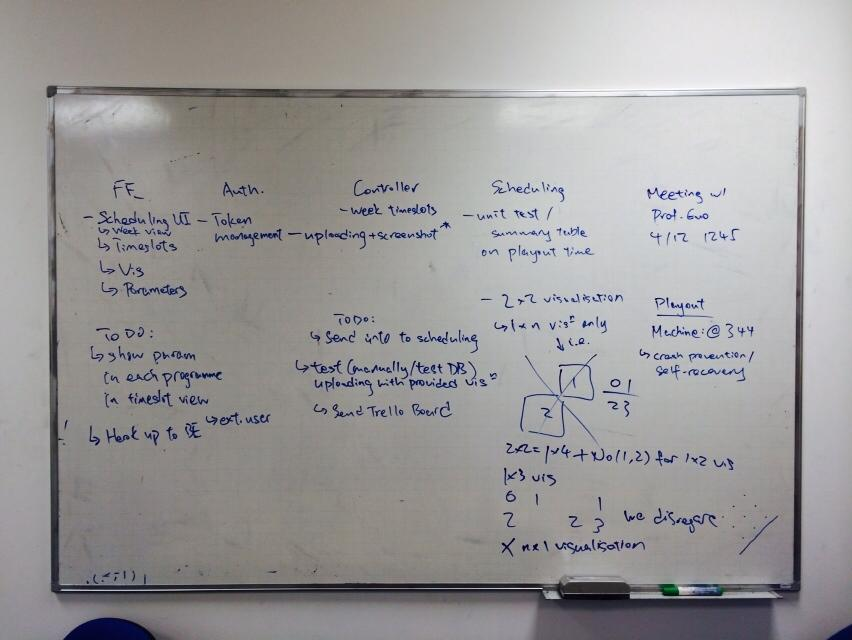
\includegraphics[width = \textwidth, trim = 1.2cm 1.5cm 1.2cm 2.5cm, clip]{./evaluation/meeting-board.jpg}
  \end{minipage}
  \caption{Meeting notes with group progress and feedback from David (our supervisor) after sprint cycles 2 (left) and 4 (right).}
  \label{fig:meetingboard}
\end{figure}

Furthermore, with the aid of Jenkins, we are able to give the address of our ``release VM'' to David, where he can see the latest working version of the project. From this, David can constantly evaluate and provide feedback on our project features through all stages of development.

\subsection{Feedback handling}

Upon receiving feedback from our stakeholders, mainly from our supervisor, we handled them depending on their nature:

\begin{itemize}

  \item Change in minor details of a feature/design: \\
        Usually happening in the prototype stage, they include changing font size/colour and displaying some extra information on a screen. As these changes take only a few hours at most to implement, we took the majority of such suggestions and fitted these XS-items in the next iteration.

  \item Introduction of new, peripheral features: \\
        These include features that are related but not essential for our three main components (submission, moderation/scheduling and playout): Multiple default playout lists, playing videos with linked themes consecutively, buttons to copy and paste previous timeslots, etc. \\
        However, due to time limitations, we chose to integrate only one or two small-sized features into our planned implementation. The rest of the suggested features were put into an ``extra feature" list, which we only considered implementing after basic versions of the main components are completed. This ensures that we can produce a minimal product at the very least before our planned deadline.

  \item Major changes in feature implementation: \\
        As a result of differing assumptions, the feedback necessitates the changing of what we have already implemented. For instance, we were required to change the priority rules in our scheduling algorithm. When this happens, we spend a significant portion of the weekly meeting to clarify the assumptions that our supervisor has made, and try to combine them with our own assumptions and implementations. This feedback has sometimes resulted in some or all of our code being scrapped, but it generates a product which is more useful to our stakeholders.

\end{itemize}

In all cases, we have communicated with the personnel that provided the
feedback with justification on our decisions. For example, we told
our supervisor that we are happy to accede to his request of adding a button which copies previous timeslots as we rate it as a S-sized task which can fit into the planned iteration, but his request for linked videos to be scheduled to be screened consecutively would delay our plans, and thus should be considered only after the entire system is implemented minimally.

\section{Product Requirement, Value \& Impact}

In the first week of embarking on our project, we met with our supervisor to highlight the initial components required. At first, these were general
requirements including:

\begin{itemize}

  \item Stakeholder requirements resembling user stories (e.g. a user is allowed to submit scientific visualisations and/or advertisements, as well as to state his/her preference(s) on playout).

  \item System/Interface requirements - what users expect it to be able to do based on the user stories above (e.g. The scheduling system should schedule items to play out in rotation, so that passers-by will not be bored by the ``fixed" playout sessions).

\end{itemize}

\begin{figure}[H]
  \centering
    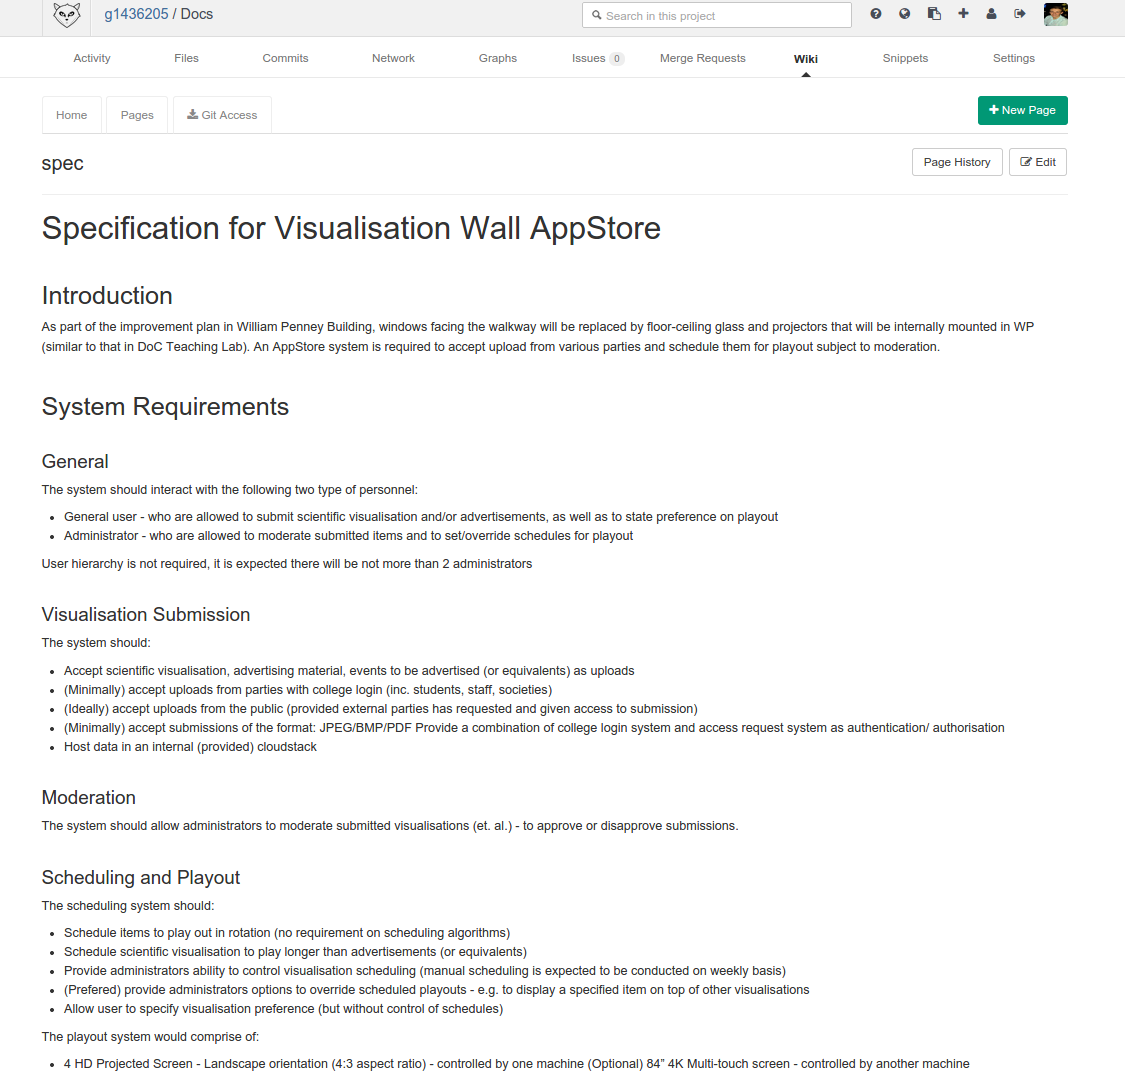
\includegraphics[width = 0.9\textwidth, trim = 0 15cm 0 5cm, clip]{./evaluation/specs.png}
  \caption{Initial specifications (partial) on shared repository.}
  \label{fig:specs}
\end{figure}

In the following weeks, we then clarified and expanded on these requirements as a group. This allowed us to discuss the implementation and technical details of specific features.

\subsection{Value Proposition}

We also further clarified our understanding of stakeholders and how our system creates value for them via multiple value proposition canvasses. Figure \ref{fig:valpropcanvas} shows the canvas for the Imperial Data Science Institute, which our supervisor is associated with. It includes a customer profile with a list of jobs, gains and pains, and corresponding products/services, gain creators and pain relievers (value map). Some of the gains/pains of the institute, along with their creators/relievers are as follows:

\begin{itemize}

  \item Gain: Makes the walkway more interesting (by showing visualisations to passers-by)

  \item Pain: Requires a large number of visualisations (relieved by inviting users to submit visualisations)

  \item Gain: Creates income opportunities (by showing adverts)

  \item Pain: Attracts inappropriate submissions from users (relieved through admin moderation)

\end{itemize}

The canvasses enable us to disregard features that deliver low or no value, and make more reasonable assumptions about our stakeholders. We believe that the latter has resulted in fewer problems for us when we began our product validation, detailed in Section \ref{sec:validation}.

\begin{figure}[H]
   \begin{center}
      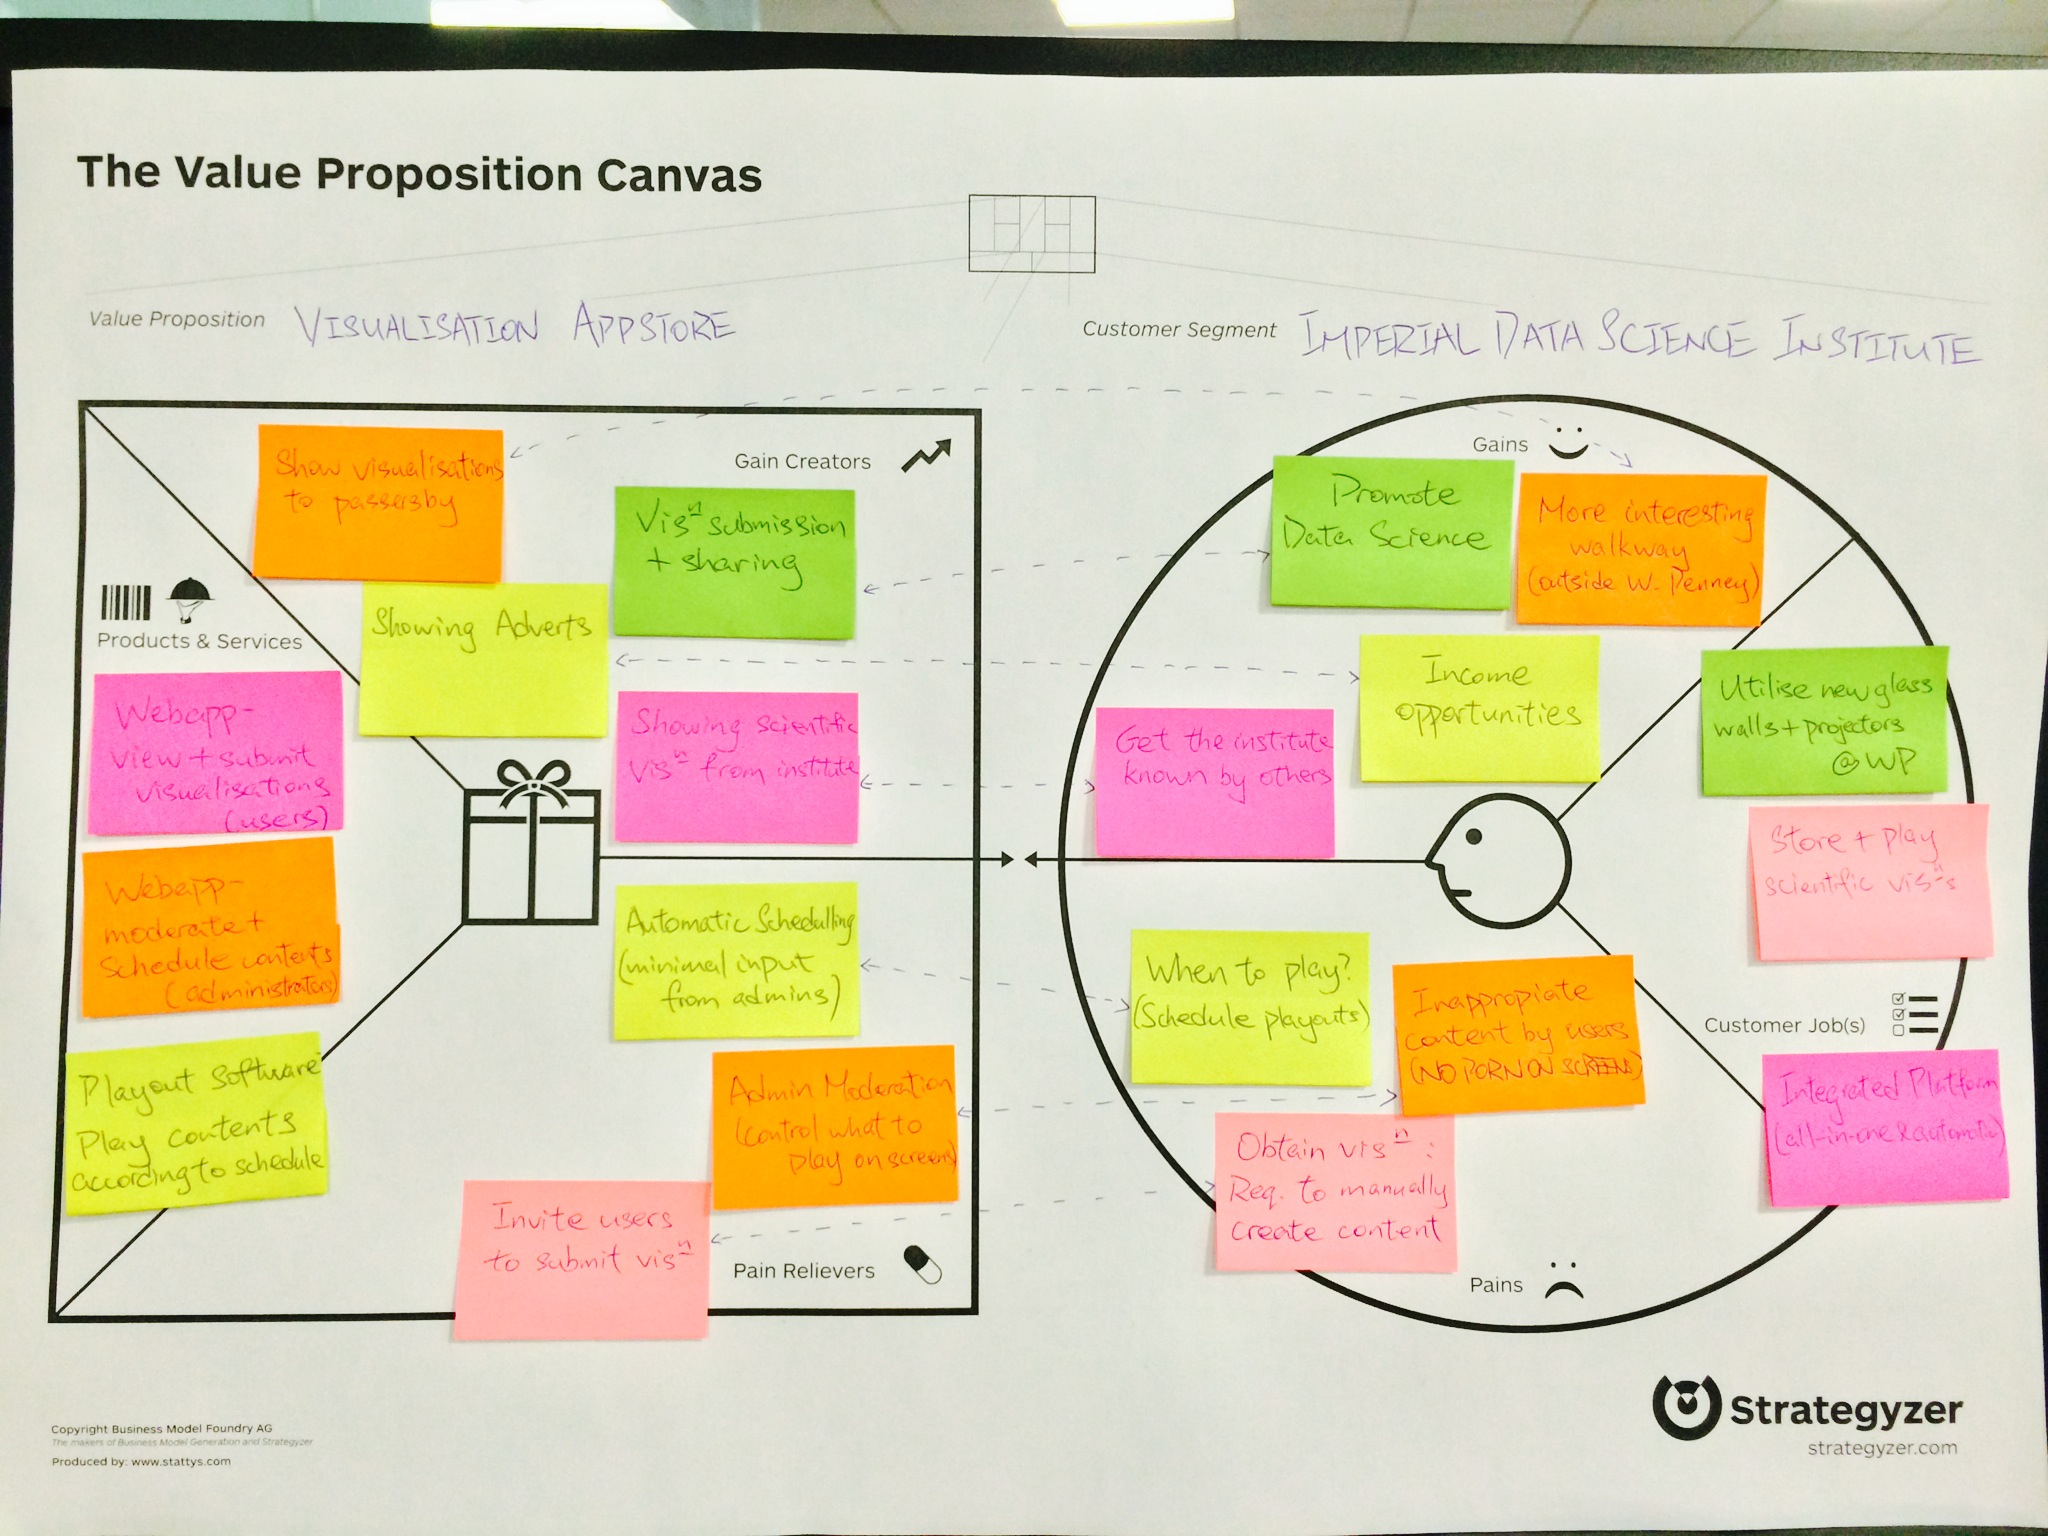
\includegraphics[width = 0.9\textwidth, trim = 1cm 6.5cm 1cm 4.5cm, clip]{./evaluation/value_prop_canvas.jpg}
   \end{center}
   \caption{Value proposition canvas for our client (Imperial Data Science Institute).}
   \label{fig:valpropcanvas}
\end{figure}

\section{Task Management}
%TODO: if required to expand

During development, we constantly looked at the requirements from all of our stakeholders, which we stored in a shared document. In our weekly scrums, we presented the work that we have done to one another and discussed whether the project is on the right track.

We prioritised tasks on our Trello board using different columns. In addition, we constantly communicated both face-to-face and online, to make sure that group members are implementing assigned tasks at the right times. We also used the Trello board actively to update the rest of the group when tasks have been completed, hence saving us the trouble of constantly asking the rest of the group or looking at code to find out if a feature has already been implemented. When appropriate, group members working on the backend used an internal wiki on Gitlab to provide information about routing, controller actions, and parameters. 

\begin{figure}[H]
  \begin{minipage}{0.49\textwidth}
    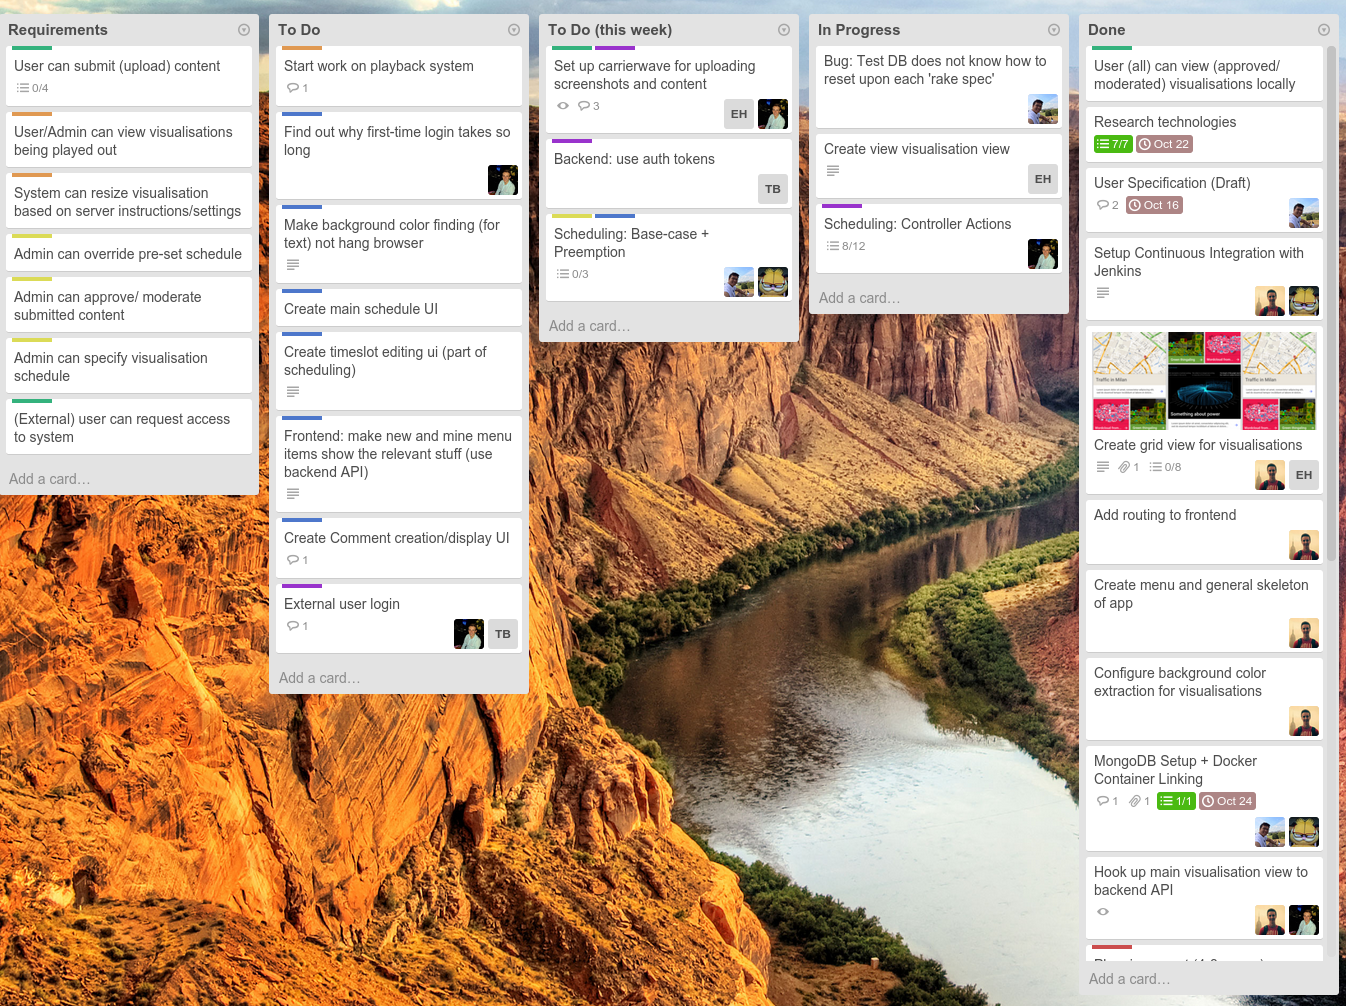
\includegraphics[width = \textwidth]{./evaluation/trello-columns.png}
  \end{minipage}
  \begin{minipage}{0.49\textwidth}
    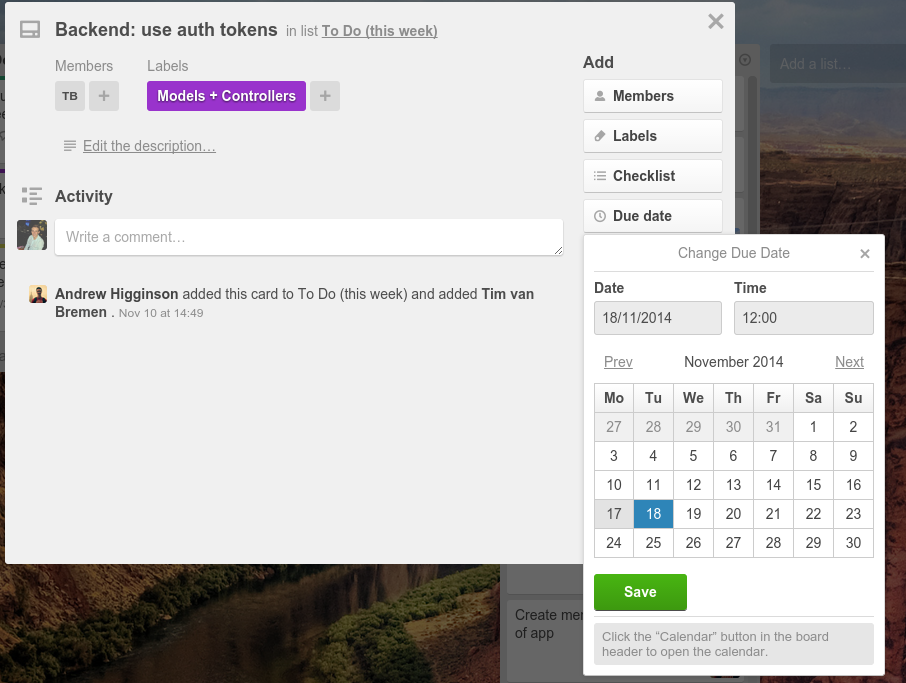
\includegraphics[width = \textwidth]{./evaluation/trello-due-date.png}
  \end{minipage}
  \caption{Priority columns on our Trello board (left), and \\ setting a due date for a particular task (right).}
  \label{fig:trello}
\end{figure}

\subsection{Story Splitting}

While some of our project requirements can be completed within a few hours, other features are unlikely to be completed within one iteration. In such cases, we split the features into multiple units and implement them in different iterations based on their priority.

An example can be found in the following user story:
\begin{center}
``\textit{As a user, I want to access the platform via a set of credentials so that I can upload visualisations (user)/perform moderation and scheduling (administrator).}'' \\
\end{center}

We considered this task to be technically challenging. Hence, we split it into the following subtasks:

\begin{itemize}

  \item As an internal user (student/staff at Imperial), I want to access the platform via my college login so that I can upload/moderate and schedule visualisations without the need for an extra set of credentials.

  \item As an external user, I want to access the platform via some kind of access request system, so that I can share my visualisations too.

\end{itemize}

In addition to being reduced in size, splitting the story has also helped us further understand the needs of different groups of users. As such, we decided to implement the former requirement first, as some of our team members have had experience on working with the college login system, hence allowing the requirement to be fulfilled in a shorter time. The latter requirement was then scheduled to be carried out in parallel with the mentioned features.

\subsection{Spikes - Experiments with new technologies}

Throughout development, we also devoted a small proportion of time to experiment on technologies involved in later iterations. This allows us to better understand the potential complications that we will face and react accordingly.

While we planned to implement the playout system only in iterations 5 and 6 (the last two iterations), investigation on relevant technologies, including Qt and its adapters, were made from iteration 2. Preliminary research allowed us to confirm that 2 weeks would be a reasonable estimate in system implementation. Furthermore, we believe that the investigation would result in a more gentle learning curve, and reduces the risk for development grinding to a halt as team members will at least have some basic knowledge on Qt, and some code segments will be produced.

However, not all spikes bring good news - investigation on Kerberos login libraries has revealed that the adapter for Flask (with Python) is actually broken, forcing us to scrap the entire implementation. Nonetheless, the spike allowed us to switch our choice of development language early and avoid incurring high costs further into development.

\section{Building the right thing - Assumption Validation} \label{sec:validation}

Given the tight deadlines for the entire project, we agreed to collect
user feedback as soon as the project commenced. This ensures that we are building the right product for our stakeholders.

\subsection{UI mockups/ prototypes} \label{sec:uimockup}

Before implementing a particular part of our project, we begin with creating mockups (Figure \ref{fig:mockup}). These can be produced in a relatively short time, and allows us to quickly think through the design of our project, without being tied down to any implementation details. After completion, we show the mockups to the main stakeholder in the project i.e. our supervisor, who gives us feedback. For example, he mentioned that it will be a good idea to show the priorities associated with each visualisation in the timeslot views, even if the visualisation is not selected after viewing the mockups.

Once we have settled on a general design, we complete the main implementation of the UI within that week's sprint cycle, but only up to the point where we can see how it will be used. As it is not interacting with the backend at this point, small changes are easily implemented, with the following week's sprint cycle involving ``hooking'' up this UI prototype with our backend.

We also made sure that this prototype is seeded with some dummy/representative data in some way, so that it is clear how each part of the project will operate in practice.

\begin{figure}[H]
   \begin{center}
      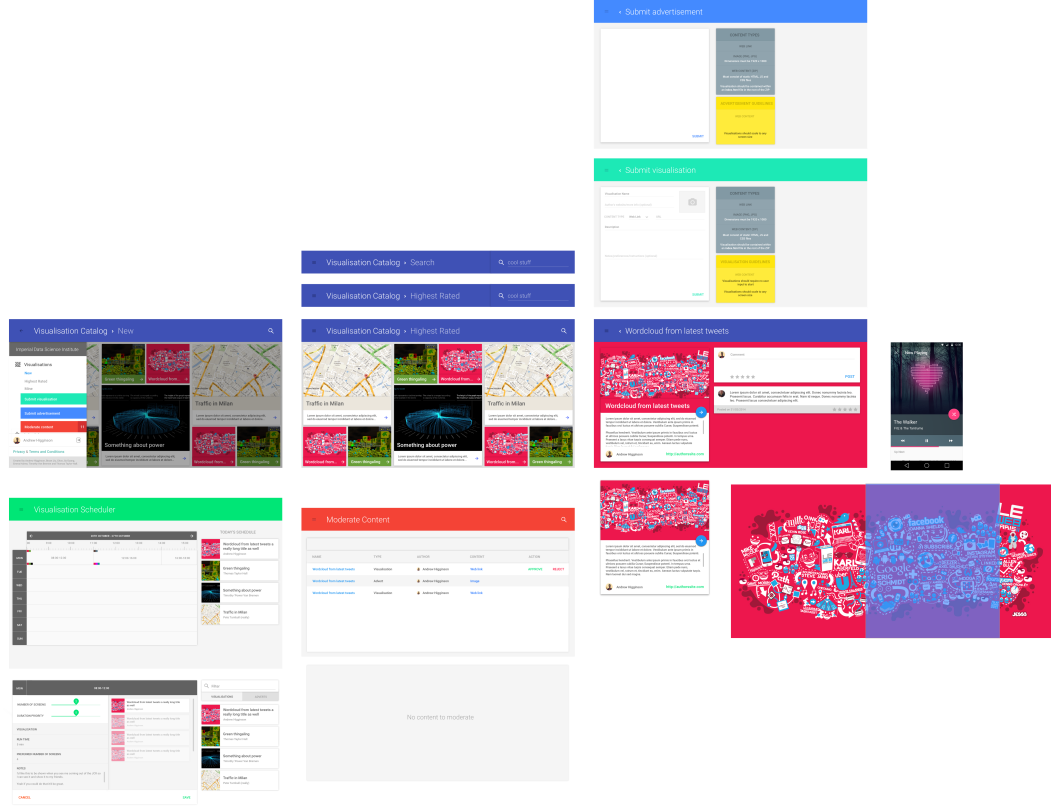
\includegraphics[width = 0.9\textwidth, trim = 0 0 0 0cm, clip]{./evaluation/mockup.png}
   \end{center}
   \caption{Mockups on User Interface}
   \label{fig:mockup}
\end{figure}

\subsection{Requirements on intangible ideas}

Compared to UIs which users can see and feel, we believed that uncovering the client's assumption on playout scheduling via mockups or prototypes will not be feasible as the scheduling algorithm is mainly rule-based. Instead, we delivered our ideas to our supervisore with whiteboard illustrations, and recorded his feedback.

Throughout these discussions, we uncovered several assumptions made by our supervisor, one of which is expecting the scheduling algorithm to ensure that playout time is directly proportional to metric set by administrators. In response, we have created additional unit tests to incorporate such requirements in our scheduling algorithm.

\begin{figure}[H]
  \begin{minipage}{0.46\textwidth}
      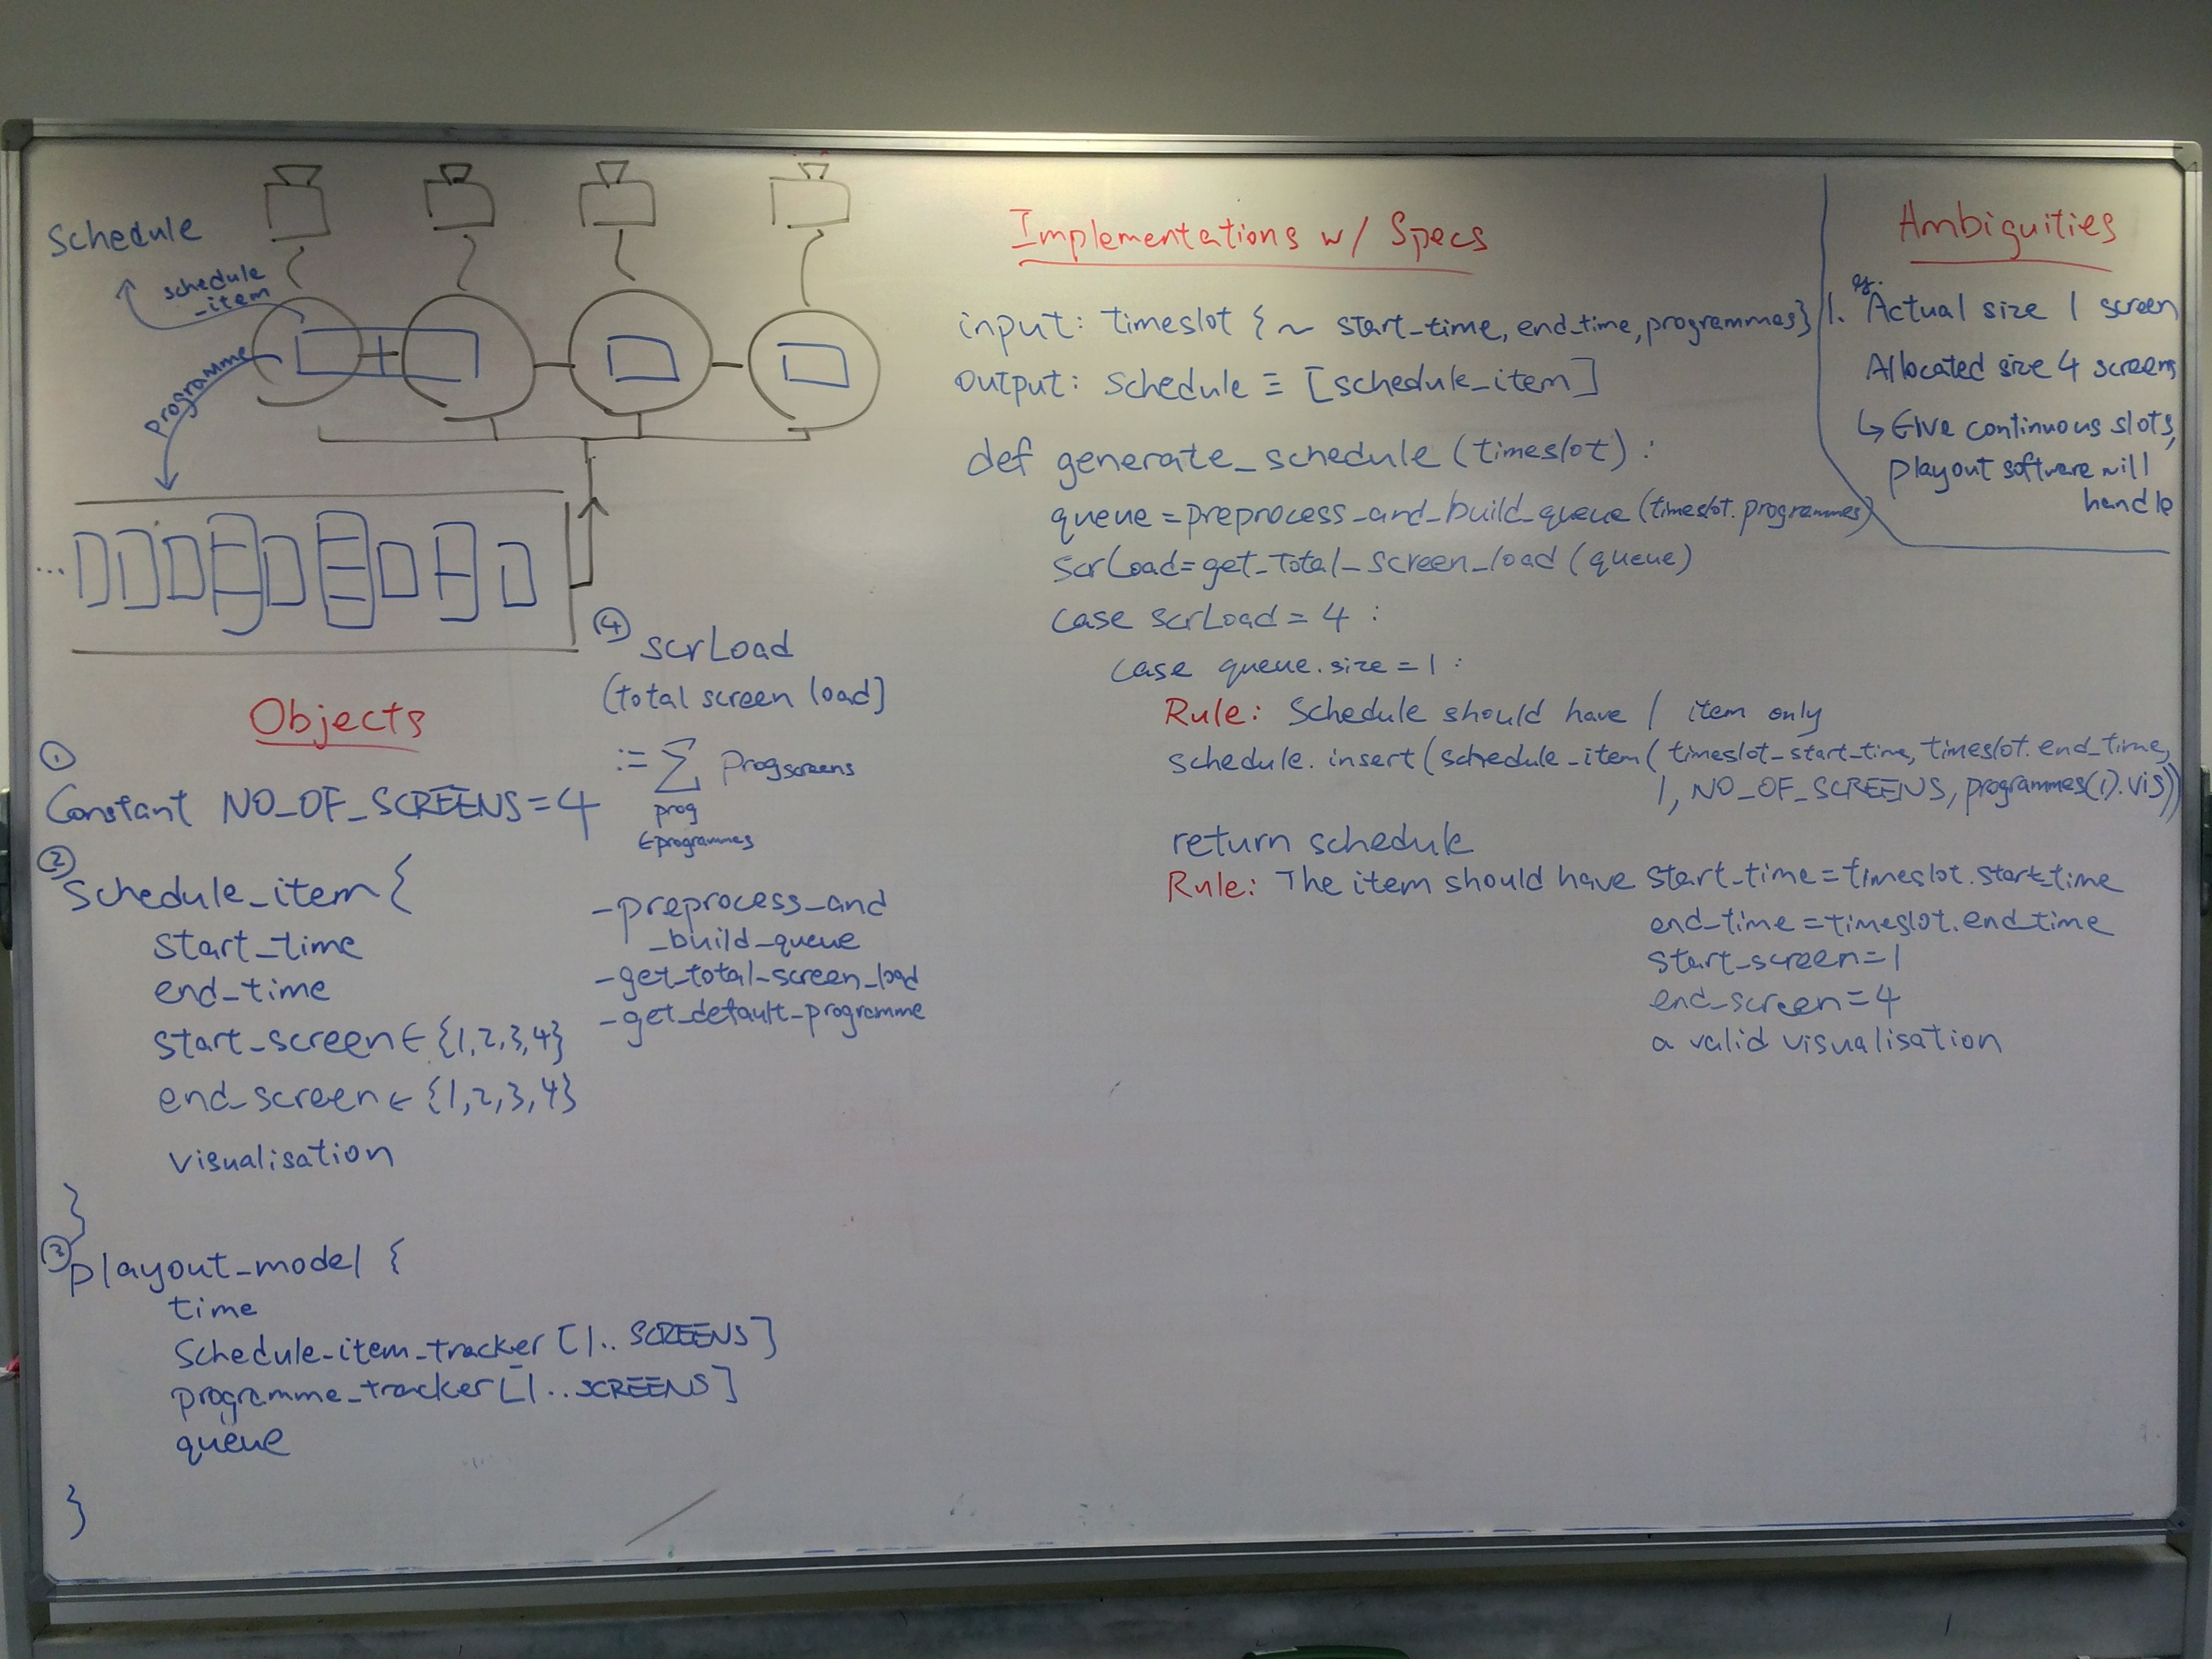
\includegraphics[width = 0.99\textwidth, trim = 0 1cm 0 1.5cm, clip]{./evaluation/scheduling_whiteboard.jpg}
  \end{minipage}
  \begin{minipage}{0.53\textwidth}
      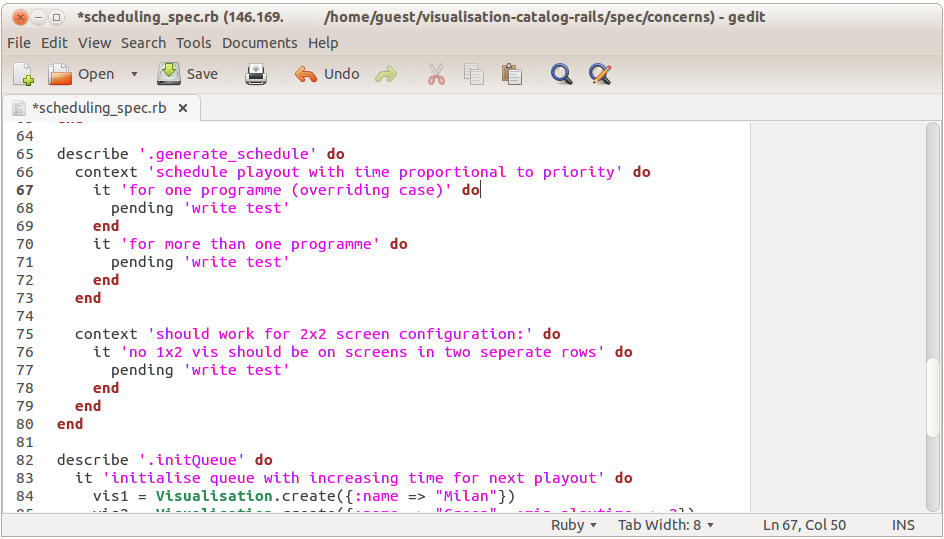
\includegraphics[width = 0.99\textwidth]{./evaluation/scheduling_spec.png}
  \end{minipage}
  \caption{Capturing scheduling requirements on whiteboard (left), \\ and subsequently via RSpec unit tests (right)}
 
\end{figure}

\subsection{User testing}

We also conducted implicit user tests during demonstrations of new features, where we asked our supervisor to complete certain tasks with minimal instructions and guidance (e.g. to navigate to the visualisation scheduling page and schedule some visualisations for playout).

Such testing allowed us to learn what is evident to us but obscure to our users. For example, in one of our demonstrations, we observed that our supervisor made multiple pauses when asked to navigate to the moderation and scheduling pages. This indicated that the icon showing the user menu may not be obvious enough to users, and the description for menu items may not be clear enough. Based on such observations, we changed the size of the ``show menu'' button, and also explored the effect of various font colours on the user menu.

We are planning to extend this user testing to include more potential users, especially those that are ranked second in our list of stakeholders, such as staff and students who may use the platform to submit and 
view visualisations.

\section{Evaluation}

As a group, we are constantly evaluating the correctness of our project by 
unit and system tests after a feature is implemented via RSpec.

\subsection{Validated learning \& Pivoting}

As mentioned in Section \ref{sec:uimockup}, producing mockups and prototypes with representative data and obtaining feedback based on them allowed us to 'pivot' many times with minimal reimplementation overhead. It also allows us to identify problems or learn more about the issues that we are trying to solve, before we write large volumes of code which may end up to be not useful. Moreover, this lean approach \textbf{encourages us} to pivot more often, as there is no reason not to do so.

\subsection{Project progress}

Quantitatively, we evaluated our project by ticking off our initial requirements. Also, we used the system ourselves, from both the user and administrator perspectives, to evaluate the project from both our stakeholders' points of view. This includes uploading visualisations and viewing other visualisations as a user, and moderating and scheduling visualisations as an administrator.

Using our Trello board and version control, we can easily see by whom each feature has been implemented. To improve our teamwork for future group projects, we will sit down as a group and describe our strengths and weaknesses in this project.

% TODO: get externals to evaluate, people from data science institute? 

% TODO: stuff from eval lecture

% TODO: metrics: move trello to here



\end{document}
